\section{Experiments}

\subsection{Datasets}

\subsubsection{Experimental datasets}

To our knowledge, there's no existing large scale database of annotated X-ray
single particle images categorized by biological/chemical samples.  The Coherent
X-ray Data Bank (CXIDB) serves as ``a permanent public repository of data from
coherent X-ray sources" \cite{maiaCoherentXrayImaging2012}.  Table \ref{tb: SPI
experiments} is a list of all SPI experiments documented on CXIDB.  We decide to
use the raw data collected in experiment amo06516
\cite{liDiffractionDataAerosolized2020}, part of which are also available by
checking out CXIDB ID 156.  One major difference between raw data and deposited
data is that raw data contain a considerable amount of \textit{non-sample-hit}
images, which are important for real-time SPI classification tasks.  For data
labelling, we created a GUI tool (\url{https:
//github.com/carbonscott/hit-labeler}) that can label hits from multiple sources,
including raw data through \textit{psana} \cite{damianiLinacCoherentLight2016}
and HDF5 files from CXIDB.  In total, we labelled {\color{red}xxx}
\textit{single-hit}, xxx \textit{multi-hit} and xxx \textit{non-sample-hit}.  

\begin{table}
\centering
%% \renewcommand{\arraystretch}{1.2}
\resizebox{1.0\textwidth}{!}{
    \begin{tabular}{  | l l l | }
        \hline
        CXIDB ID & Light Source & Sample \\
        \hline
        001      & LCLS         & Mimivirus                                                       \\
        002      & LCLS         & Mimivirus                                                       \\
        003      & FLASH        & FIB etched 20-nm-thick silicon nitride membrane                 \\
        004      & ALS          & Gold labeled frozen dried Saccharomyces cerevisiae yeast cells. \\
        005      & ALS          & Gold labeled frozen dried Saccharomyces cerevisiae yeast cells. \\
        006      & ALS          & Gold labeled frozen dried Saccharomyces cerevisiae yeast cells. \\
        007      & ALS          & Gold labeled frozen dried Saccharomyces cerevisiae yeast cells. \\
        008      & ALS          & Gold labeled frozen dried Saccharomyces cerevisiae yeast cells. \\
        009      & FLASH        & Iron Oxide Ellipsoids                                           \\
        010      & LCLS         & Nanorice                                                        \\
        011      & LCLS         & Magnetosomes                                                    \\
        012      & LCLS         & Tobacco mosaic virus                                            \\
        013      & LCLS         & T4 bacteriophage                                                \\
        014      & LCLS         & Paramecium bursaria Chlorella virus                             \\
        019      & LCLS         & Airborne Particulate Matter (Soot)                              \\
        020      & LCLS         & Clusters of Polystyrene Spheres                                 \\
        025      & LCLS         & Carboxysomes                                                    \\
        026      & LCLS         & Cyanobium gracile                                               \\
        027      & LCLS         & Synechococcus elongatus                                         \\
        028      & ALS          & 50 nm colloidal gold particles                                  \\
        030      & LCLS         & Mimivirus                                                       \\
        036      & LCLS         & Rice Dwarf Virus                                                \\
        037      & LCLS         & Cyanobium gracile and Synechococcus elongtatus                  \\
        056      & LCLS         & Omono River Virus                                               \\
        057      & LCLS         & Gold core and palladium shell nanoparticles                     \\
        058      & LCLS         & Coliphage PR772                                                 \\
        078      & LCLS         & RNA polymerase II                                               \\
        084      & ESRF         & Gold structure (largest diameter about 1.1 um)                  \\
        088      & LCLS         & PR772                                                           \\
        119      & LCLS         & Sucrose                                                         \\
        146      & FLASH        & Xenon nanoclusters                                              \\
        155      & LCLS         & Melbournevirus                                                  \\
        156      & LCLS         & Coliphage PR772                                                 \\
        \hline
    \end{tabular}
}
\caption{All SPI experiments documented on CXIDB.}
\label{tb: SPI experiments}
\end{table}


\subsubsection{Simulated datasets}

Similarly, there's no existing large scale database of annotated SPI images
generated by physics-based simulation.  To investigate generalizability of our
SPI classifier, it's essential to have a large dataset of simulated SPI images.
We resort to \textit{skopi} \cite{peckSkopiSimulationPackage2021}, a GPU-based
program for simulating diffractive images from noncrystalline biomolecules, for
concurrently simulating high-resolution SPI scattering and providing accurate
labels in an automated manner at scale.  

Our primary interest is to explore the model generalizability on \textit{large}
single particles, considering the state-of-art resolution ever reached in an SPI
experiment is still at the nanometer level ($>$ 10 $nm$) {\color{red} (need to
fact-check)} unlike in protein crystallography that studies biological
structures at the angstrom level.  PDB statistics offers direct insights into
PDB data distribution by molecular weight (\url{https:
//www.rcsb.org/stats/distribution-molecular-weight-structure}).  We focus on
\textit{large} particles with molecular weights over 380 $KDa$.  Fig. \ref{fig:
num atom per bio assem} describes the population frequency of the atom numbers
per biological assembly with each area representing 50 PDB items.  The atom
numbers spread across three orders of magnitudes ($10^4\text{-}10^6$).  96.0\%
of \textit{large} particles have $10^4$ atoms, and only 1.2\% have massive
$10^6$ atom numbers. Simulated datasets are generated by setting the detector
distance at 100.0 $mm$ and photon energy at 1.660 $keV$.  

% Insert the figure HERE and TOP..
\begin{figure}
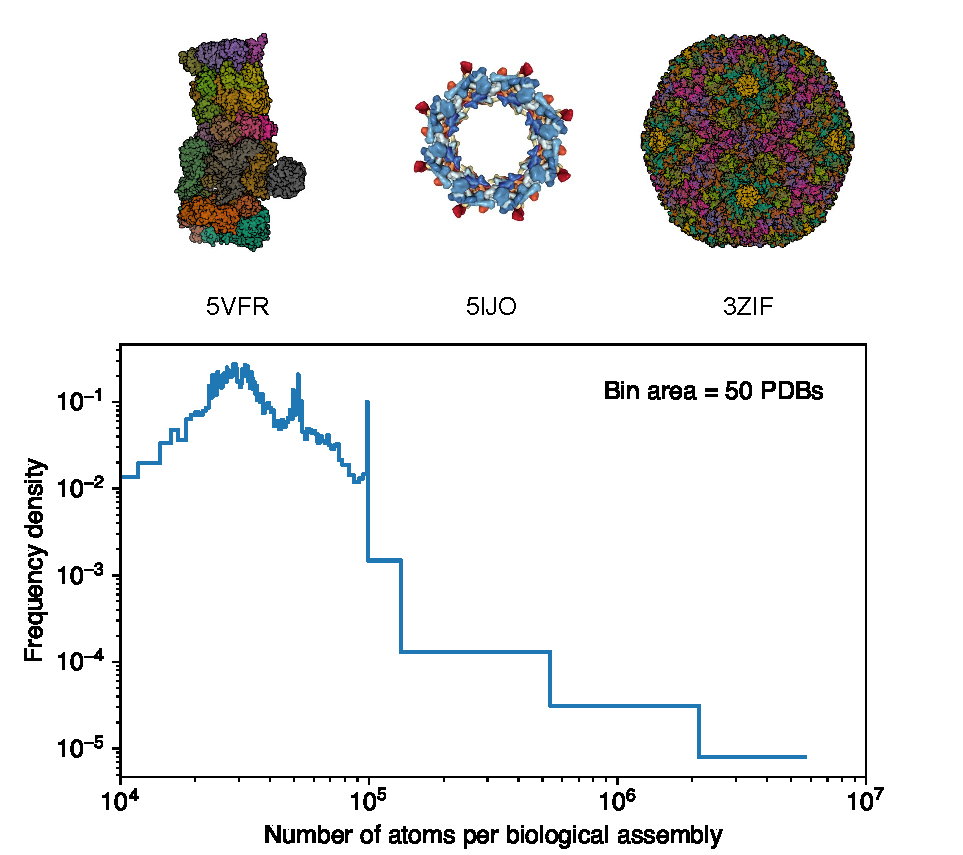
\includegraphics[width=1.0\textwidth,keepaspectratio]
{./figures/num_atom_per_bio_assem.pdf}
\caption{Number of atom per biological assembly. {\color{red} Need to indicate where
those molecular graphs are from.}}
\label{fig: num atom per bio assem}
\end{figure}


\subsubsection{Image mode, mosaic mode and panel mode}

One major constraint in real-time scenario is that we might not have a complete
view of a scattering pattern assembled from pixel areas of individual detector
panels.  We thus consider three different modes in dataset curation: (1) Image
mode, where information from all detector panels is consolidated according to
their respective physical locations; (2) Mosiac mode, where information from
serveral detector panels are combined without acknowleding any geometric
relations among panels;  (3) Panel mode, meaning that only pixel contents in a
single panel during a exposure is visiable to our model.  Image assembly is
trivial in offline applications, but can be complicated in real-time
applications.  Detector readouts from various panels require extra delay to
synchronize and image assembly itself might not be instantaneous, potentially
bottlenecking the FPS (frame per second) during X-ray exposure. Likewise, Mosic
mode allows the use of fewer panels, but is not able to get around the
synchronization issue either.  Conversely, panel mode is currently best suited
for real-time applications, since it doesn't have the constraints of
synchronization delay or image assembly.  One noticable limitation, though, is
that partial information about a scattering pattern on a single panel can
undermine the performance of classification.  On a side note, detectors made of
small panels might not be a good choice for high-speed SPI imaging.  


\subsubsection{Data augmentation for synthetic dataset}

% Random zooming: detect at different detector distances.

Since synthetic datasets are constructed by simulation, there are plenty for
model training on demand.  We find data augmentation still quite valuable in
providing variations caused by changes in detector distance.  For example, it is
expensive to re-simulate scattering patterns using the same particle with the
same conditions but a different detector distance.  Instead, we choose to
randomly zoom in a scattering pattern that is effectively the same as increasing
detector distance.  Zoom-out is technically more difficult to achieve for
missing pixels need to be filled in around the boarders of the original image.
We think zooming-out is not necessarily a scenario we should take into account,
as it will hurt the model performances and should be fixed from the data
collection stage, e.g. users in beamlines can adjust the detector distanecs so
that the diffraction pattern has an adequate size.  


\subsubsection{Performance on experimental data}

xxxx

\begin{figure}
\centering
\includegraphics[width=\textwidth,height=0.8\textheight,keepaspectratio]
{example-image}
\caption{Fast convergence}
\label{fig:fast_convergence}
\end{figure}

\begin{figure}
\includegraphics[width=\textwidth,height=0.8\textheight,keepaspectratio]
{example-image}
\caption{Regularization on performance}
\label{fig:regularization_on_performance}
\end{figure}


\begin{figure}
\includegraphics[width=\textwidth,height=0.8\textheight,keepaspectratio]
{example-image}
\caption{Confusion matrix (no regularization)}
\label{fig:confusion_matrix_no_reg}
\end{figure}

\begin{figure}
\includegraphics[width=\textwidth,height=0.8\textheight,keepaspectratio]
{example-image}
\caption{Confusion matrix (with regularization)}
\label{fig:confusion_matrix_with_reg}
\end{figure}

Nanorice and T4 phage

\subsubsection{Performance on synthetic data}

xxxx

\begin{figure}
\includegraphics[width=\textwidth,height=0.8\textheight,keepaspectratio]
{example-image}
\caption{PDB split vs performance}
\label{fig:confusion_matrix_with_reg}
\end{figure}

\begin{figure}
\includegraphics[width=\textwidth,height=0.8\textheight,keepaspectratio]
{example-image}
\caption{Confusion matrix (10\%)}
\label{fig:confusion_matrix_with_reg}
\end{figure}

